\begin{tikzpicture}
	\begin{axis}[
        xlabel={Aufgabe},
		ylabel={Zeit in s},
		title=Zeit pro Tester und Aufgabe,
		ybar,
		bar width=0.15cm,
		symbolic x coords={L2.6, L2.7, L3.1, L3.2, L3.3, L3.4, L3.5},
		xtick={L2.6, L2.7, L3.1, L3.2, L3.3, L3.4, L3.5},
		width=0.89\textwidth,
		height=0.9\textheight,
		legend style={
			at={(1.15, 0.0)},
			anchor=south,
			column sep=1ex
		}
	]
	\addplot[style={lime,fill=lime}] coordinates {(L2.6,0)(L2.7,37)(L3.1,0)(L3.2,0)(L3.3,0)(L3.4,0)(L3.5,0)};
	\addplot[style={green,fill=green}] coordinates {(L2.6,20)(L2.7,3)(L3.1,5)(L3.2,5)(L3.3,20)(L3.4,20)(L3.5,0)};
	\addplot[style={blue,fill=blue}] coordinates {(L2.6,0)(L2.7,0)(L3.1,0)(L3.2,0)(L3.3,0)(L3.4,0)(L3.5,0)};
	\addplot[style={red,fill=red}] coordinates {(L2.6,0)(L2.7,0)(L3.1,0)(L3.2,0)(L3.3,0)(L3.4,0)(L3.5,0)};
	\addplot[style={purple,fill=purple}] coordinates {(L2.6,120)(L2.7,30)(L3.1,30)(L3.2,30)(L3.3,30)(L3.4,30)(L3.5,120)};
	\addplot[style={violet,fill=violet}] coordinates {(L2.6,60)(L2.7,60)(L3.1,60)(L3.2,60)(L3.3,60)(L3.4,60)(L3.5,60)};
	\legend{Hönig, Bär, Sukhankova, Schanck, Naumann, Leyer}
	\end{axis}
\end{tikzpicture}